\section{多股共端场路与均流判据}
\label{chapter:04}

% block-id: 04.common.heading
\hypertarget{04.common.heading}{}
\subsection{共端场路与复电流均流条件}

% block-id: 04.common.p1
\hypertarget{04.common.p1}{}
共同端点、股线支路与回流的关系见 图~\ref{fig:common_terminal}。令 Z 为指定线性模型的耦合阻抗矩阵，e 为独立外场引起的感应项，i 为各股复电流，V 为公共端电压。端口方程 Z i+e=V1 与总电流条件 1\(^{\mathrm T}\)i=It 共同构成 \eqref{eq:E04}。求解该增广系统可同时得到幅值和相位，等流值 It/N 用于比较求得的电流分布。

% block-id: 04.common.p2
\hypertarget{04.common.p2}{}
在增广系统具有唯一解时，令 i=(It/N)1 可知：等流解存在，当且仅当向量 (It/N)Z1+e 的所有分量相同。将该向量投影到与 1 正交的子空间，便得到 \eqref{eq:E05}。无独立外场时，条件简化为 Z 的各行和相同；存在外场时，感应项也参与决定均流。该判据给出了所选阻抗模型与端接条件下的充要条件，便于将几何换位的作用具体落实到耦合矩阵及感应项的变化上。

% block-id: 04.common.p3
\hypertarget{04.common.p3}{}
二维共端 FEM 将公共轴向端场与 Az 自由度联合求解。导体内按 Jz=σ(v−u) 恢复电流密度，其中 v 与保存变量 u 均以 V/m 表示，回流导体使用相应的端场。电流和损耗由带材料标记的线性三角形积分，坐标由 mm 转换为 m 后计算面积。由此得到的逐股复电流、束内损耗、回流损耗及铜面积，与原始场路结果独立核对；空气区域与各导体区域分别处理。

% block-id: 04.sharing_derivation.heading
\hypertarget{04.sharing_derivation.heading}{}
\subsection{复电流均流条件的推导}

% block-id: 04.sharing_derivation.p1
\hypertarget{04.sharing_derivation.p1}{}
若等流解存在，将 i=(It/N)1 代入端口方程，即得向量 (It/N)Z1+e 的全部分量相同，投影条件因而必要。反之，若投影条件成立，该向量可写为某一标量 V 与 1 的乘积，等流向量同时满足端口方程和总电流约束；在增广系统解唯一时，它即为实际解，条件因而充分。数值结果以 sqrt(mean(|ik−It/N|²))/|It/N| 表示归一化复电流 RMS 偏差，并同时展示逐股幅值与相位。

% block-id: 04.coax_results.heading
\hypertarget{04.coax_results.heading}{}
\subsection{640 股直束的共端电流与损耗}

% block-id: 04.coax_results.p1
\hypertarget{04.coax_results.p1}{}
三档网格以及回流距离、外域变化共完成 23 项检查。末次网格细化的 Rac 变化为 0.011902\%，回流距离与外域变化分别为 0.000495\% 和 0.000270\%，见 图~\ref{fig:coax640_mesh}。在已检查的扰动范围内，这些变化均小于 1\% 比较目标，支持指定二维共端模型结果的数值稳定性。其适用对象为受控回流下的二维直束，实际绕制结构的有限端区与沿程耦合仍需进一步验证。

% block-id: 04.coax_results.p2
\hypertarget{04.coax_results.p2}{}
图~\ref{fig:coax640_currents} 按物理股线身份展示电流幅值和相位，It/N 为等流参照。幅值差异与相位差共同决定各股对总输运电流的贡献，因此均流程度应根据复电流评价。图~\ref{fig:coax640_fields} 给出相应的截面场分布，可将逐股统计与空间位置联系起来。对于这一沿轴向保持截面的直束，细股自身的趋肤尺度与束内磁耦合造成的集体电流分配同时存在；沿程换位的影响需另行引入位置变化。

% block-id: 04.interpretation.heading
\hypertarget{04.interpretation.heading}{}
\subsection{束内与回流能量}

% block-id: 04.interpretation.p1
\hypertarget{04.interpretation.p1}{}
640 股截面结果说明了细股自身趋肤尺度与束内集体电流分配之间的区别。外层与内层股线具有不同的磁耦合环境，共同端电压使这种差异表现为复电流的幅值和相位变化。此时直流面积给出铜利用率的基准，束内焦耳积分给出输运损耗，而回流的单独积分解释完整场路的能量分配。

% block-id: 04.quantitative.p1
\hypertarget{04.quantitative.p1}{}
640 股二维模型的实际铜截面为 \metric{coax_area} mm²。束内交流电阻为 \metric{coax_rac} mΩ/轴向m，束内损耗为 \metric{coax_bundle_loss} W/轴向m，回流损耗为 \metric{coax_return_loss} W/轴向m；分开积分明确了导体束与回流各自的热耗散。共同端轴向电场为 \metric{coax_voltage_re}+j(\metric{coax_voltage_im}) V/m。各股复电流之和恢复 20 A RMS，而归一化复电流 RMS 偏差为 \metric{coax_spread}，表明该共端直束存在显著的股间电流差异。

% block-id: 04.equation.E04
\hypertarget{04.equation.E04}{}
\hypertarget{E04}{}\begin{equation}\begin{bmatrix} Z&-\mathbf1\\ \mathbf1^T&0\end{bmatrix}\begin{bmatrix}\mathbf i\\V\end{bmatrix}=\begin{bmatrix}-\mathbf e\\I_t\end{bmatrix}\tag{4}\label{eq:E04}\end{equation}

% block-id: 04.equation.E05
\hypertarget{04.equation.E05}{}
\hypertarget{E05}{}
\begin{equation}
\begin{gathered}
Q=I_N-\mathbf1\mathbf1^T/N \\
Q\left[(I_t/N)Z\mathbf1+\mathbf e\right]=\mathbf0
\end{gathered}
\tag{5}\label{eq:E05}
\end{equation}

% block-id: 04.figure.common_terminal
\hypertarget{04.figure.common_terminal}{}
\begin{figure}[!htbp]
\centering
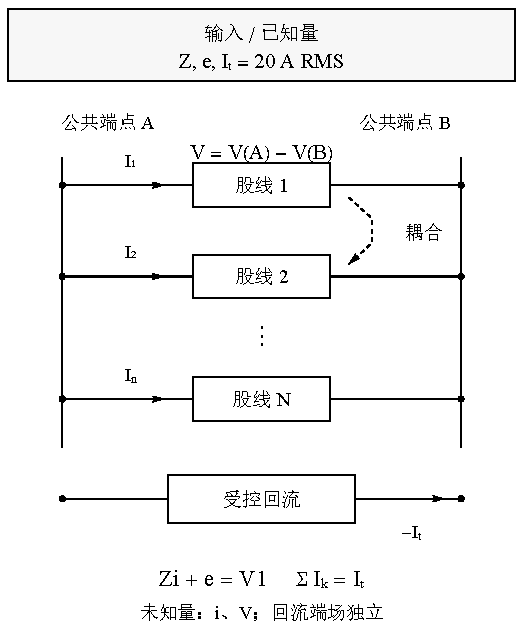
\includegraphics[width=\linewidth,height=.72\textheight,keepaspectratio]{../../assets/zh-CN/common_terminal.pdf}
\caption{多股共同端口与回流。 各股沿途绝缘，在两端并联，逐股复电流由共同端电压及总电流约束求解。耦合矩阵 Z 与激励项 e 包含指定模型中的阻抗和场作用。受控回流承担反向总电流，并具有独立的端场。图中给出已知输入及待求复电流和电压。}
\label{fig:common_terminal}
\end{figure}

% block-id: 04.figure.coax640_currents
\hypertarget{04.figure.coax640_currents}{}
\begin{figure}[!htbp]
\centering
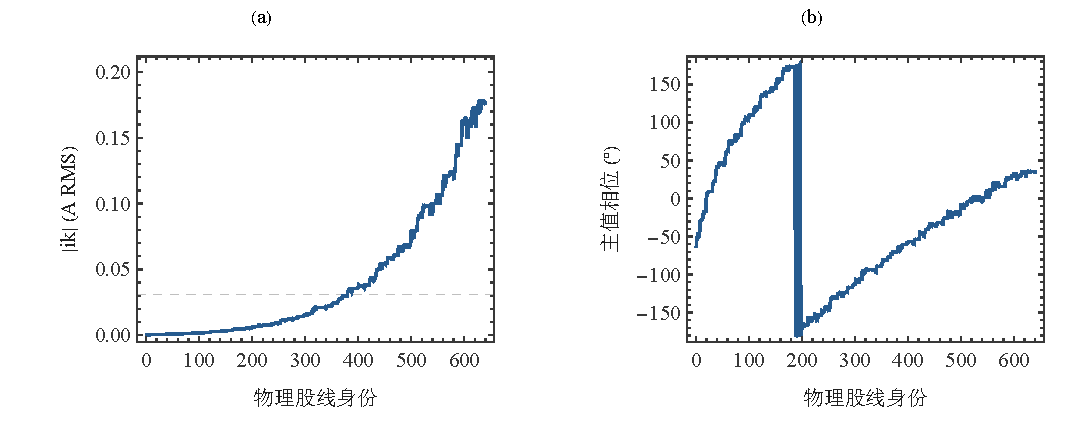
\includegraphics[width=\linewidth,height=.72\textheight,keepaspectratio]{../../assets/zh-CN/coax640_currents.pdf}
\caption{640 股共端复电流分配。 (a) 幅值；(b) 相位，按物理股线身份排列。 虚线表示 It/N 的比较参照。幅值和相位使用相同的物理股线编号。}
\label{fig:coax640_currents}
\end{figure}

% block-id: 04.figure.coax640_fields
\hypertarget{04.figure.coax640_fields}{}
\begin{figure}[!htbp]
\centering
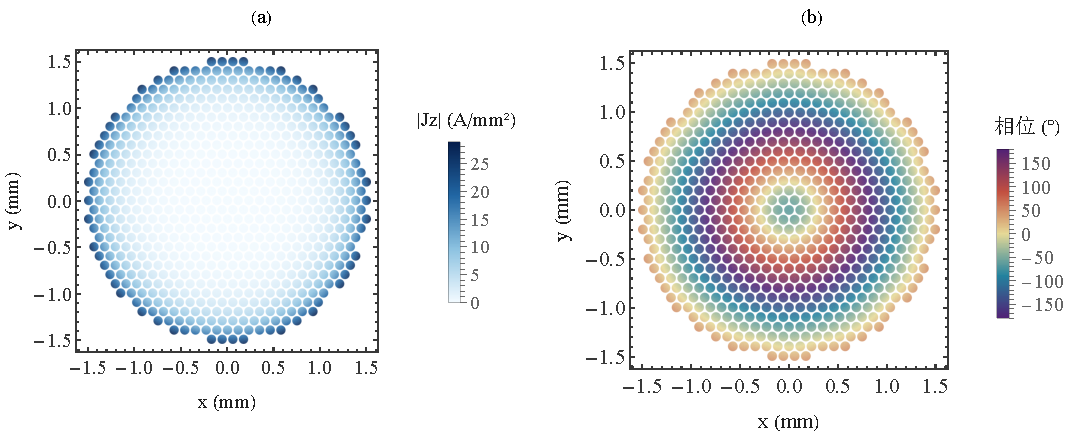
\includegraphics[width=\linewidth,height=.72\textheight,keepaspectratio]{../../assets/zh-CN/coax640_fields.pdf}
\caption{640 股二维截面电流密度。 (a) RMS 幅值；(b) 相位，材料标记识别各股。 电流按 Jz=σ(v−u) 从原节点场与端场恢复。独立功率使用线性三角形质量积分，显示采用单元中心采样。}
\label{fig:coax640_fields}
\end{figure}

% block-id: 04.figure.coax640_mesh
\hypertarget{04.figure.coax640_mesh}{}
\begin{figure}[!htbp]
\centering
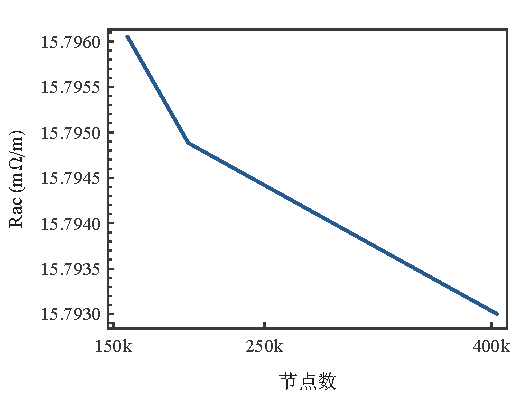
\includegraphics[width=\linewidth,height=.72\textheight,keepaspectratio]{../../assets/zh-CN/coax640_mesh.pdf}
\caption{640 股网格与边界敏感性。 各试验按网格、回流和外域分别改变一个因素。 变化以相邻指定工况的电阻差归一化。网格、回流距离与外域大小各使用独立序列。}
\label{fig:coax640_mesh}
\end{figure}
